% called by main.tex
%
\chapter{Marco Teórico}
\label{ch::capitulo5}

Hay ciertos conceptos que son fundamentales para el desarrollo e implementación del proyecto. El objetivo de esta sección es explicarlos brevemente, para permitir un mejor entendimiento del lector acerca de nuestro proceso de investigación y experimentación.

\section{Árboles de decisión}

En primer lugar tenemos aquello que es la base fundamental del algoritmo de aprendizaje supervisado propuesto a modificar, los \textbf{árboles de decisión}.

Para comprender cómo funcionan, es útil pensar en que son básicamente una serie de reglas que nos ayudan a tomar una decisión. Por ejemplo, si tuviéramos que comprar una casa, podríamos empezar a preguntarnos ¿cuál es nuestro presupuesto?, la respuesta nos lleva a casas de gama más alta o baja, luego preguntarnos, ¿cuántos ambientes necesitamos?, la respuesta nos hará descartar algunas opciones, y así sucesivamente hasta llegar a una respuesta.

Un árbol de decisión toma datos y aprende cuales son las mejores preguntas para hacerse. En el mundo de la tecnología se utilizan para tomar decisiones automatizadas en tareas de clasificación, como podría ser dar o no un crédito en base al historial crediticio de un individuo o para realizar predicciones en tareas de regresión, como predecir el precio de un hogar en base a sus características.

Entendiendo la idea de su utilidad, la estructura que tienen estos árboles de decisión es clave para comprender nuestro trabajo de experimentación. Están compuestos por nodos, que se pueden clasificar en tres tipos:

\begin{itemize}
    \item \textbf{Nodo raíz}: El nodo inicial del árbol, donde tenemos todos los datos a disposición. Buscamos a partir de este punto empezar a segmentar los datos según alguna característica, que nos ayude con nuestro propósito de tomar una decisión o realizar una predicción. Siguiendo el ejemplo de predecir el precio de una casa, podríamos dividir las casas con más de cuatro ambientes y menos o exactamente cuatro ambientes.
    \item \textbf{Nodos internos}: Los nodos internos son los que provienen de divisiones de datos anteriores, pero que también realizan una nueva separación. Luego de dividir por cantidad de ambientes podríamos dividir por más o menos de $100mt^{2}$, tanto a los hogares con más de cuatro ambientes como a aquellos con menor o exactamente cuatro.
    \item \textbf{Nodos hoja}: Finalmente, los nodos hoja son aquellos que provienen de una división de datos pero no generan nuevas particiones. Una vez que llegamos a un nodo hoja, todos los datos que cumplen con las características para haber llegado hasta ese punto en el árbol se promedian, dándonos un valor para nuestra predicción para cuando un nuevo dato ingrese en el árbol y tenga esas características. Es por ello que entonces, en el ejemplo previo, si quisiéramos predecir el precio de una casa de cuatro ambientes y $99mt^{2}$, daríamos como predicción el promedio del precio de todas las casas en nuestros datos que tenían cuatro ambientes o menos y menos de $100mt^{2}$, ya que este representa el valor esperado de precio dadas las características, según nuestra muestra de datos de entrenamiento.
\end{itemize}

En la \hyperref[figure1]{Figura 1} se puede observar un ejemplo de un árbol de decisión entrenado para predecir el promedio del valor de las casas en una zona o barrio. Para su entrenamiento contó con 16.500 datos de distintas zonas de California con las siguientes variables:

\begin{itemize}
    \item Average Income (MedInc): Ingreso promedio en la zona en decenas de miles de USD.
    \item Housing Average Age (HouseAge): Edad promedio de las viviendas en la zona, en años.
    \item Average Rooms (AveRooms): Promedio de habitaciones por vivienda en la zona
    \item Average Bedrooms (AveBedrms): Promedio de dormitorios por vivienda en la zona.
    \item Population (Population): Número total de personas que viven en el área o vecindario.
    \item Average Occupation (AveOccup): Promedio de personas por hogar en la zona.
    \item Latitude (Latitude): Latitud geográfica de la zona.
    \item Longitude (Longitude): Longitud geográfica de la zona. Complementa la latitud para la ubicación exacta de la zona en el mapa.
\end{itemize}

\begin{figure}[h]
\centering
    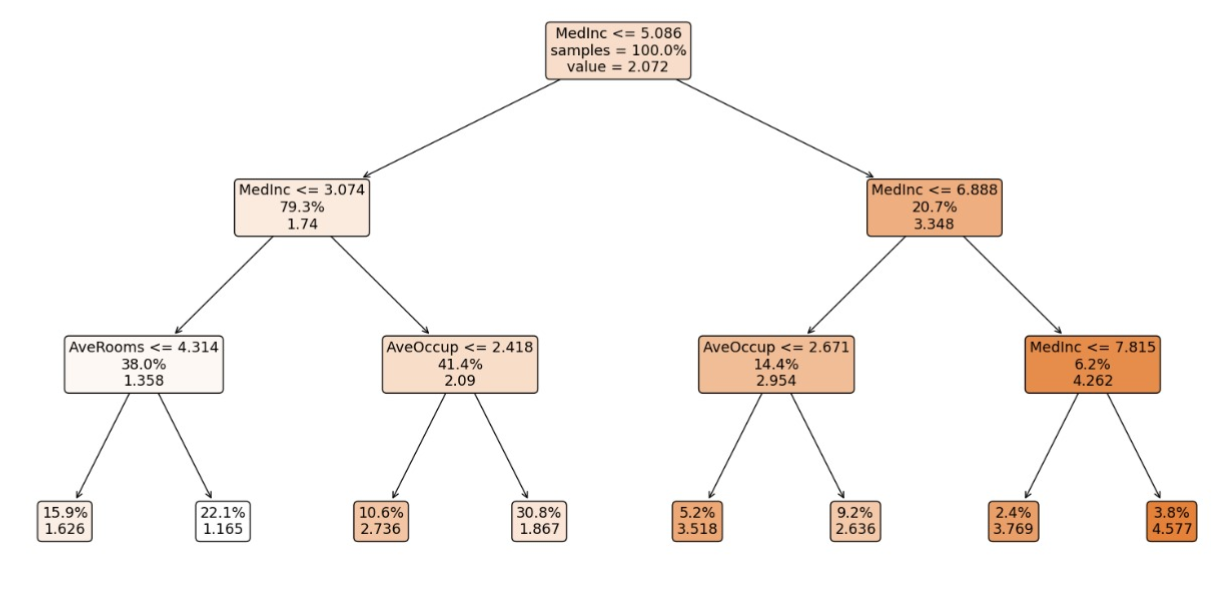
\includegraphics[width=1\textwidth]{figures/marco-teorico/tree-ilustrativo.png}
\caption{Árbol de decisión de ejemplo para predecir el precio de casas en miles de USD.}
\end{figure}
\label{figure1}

Entonces, observando el camino hasta el primer nodo hoja de la izquierda, en una zona donde el ingreso promedio es menor a $\text{\textdollar} 30740$ y la cantidad de habitaciones de las casas en promedio son menor a $4.3$, la predicción dada por el árbol es que en esa zona las casas en promedio cuestan $\text{\textdollar} 162600$.

Para determinar cuáles son las mejores divisiones para los nodos y darle un puntaje de qué tan bueno es un árbol de decisión existen distintos criterios. A lo largo de nuestro proyecto vamos a estar trabajando particularmente con problemas de regresión, es decir, dados ciertos datos, predecir un valor numérico, como el precio de un hogar. Debido a esto, utilizaremos como criterio el Error Cuadrático Medio (MSE por sus siglas en inglés), ya que es la alternativa más popular y extendida en la literatura e industria para este tipo de problemas. 

El MSE se define como el promedio de las diferencias entre las predicciones ($\hat{y_{i}}$) y los valores reales ($y_{i}$), elevadas al cuadrado:
\[
MSE = \frac{1}{n} \sum_{i=1}^{n} (y_{i} - \hat{y_{i}})^2 \,,
\]

con $n$ siendo la cantidad de datos observados.

Este criterio se utiliza para evaluar todos las posibles separaciones de datos con las características dadas (conocidas como \textit{features}). Aquella división que menor MSE da en cada paso es la división que se selecciona. Así sucesivamente hasta finalizar la construcción del árbol, que puede tener distintas normas para finalizar, como puede ser una profundidad máxima o la cantidad mínima de observaciones que debe haber en cada nodo hoja, decididas por el usuario.


\section{Random Forest}

Random Forest (RF) es un algoritmo de aprendizaje supervisado de tipo \textit{ensamble} introducido por \cite{breimanRF}, el cual se ha establecido como una herramienta estándar en el área de \textit{machine learning} dada su robustez y versatilidad a largo de diferentes aplicaciones. Básicamente este algoritmo propone, en lugar de crear un único árbol de decisión con toda la información disponible en entrenamiento, la creación de varios árboles de decisión, cada uno formado a partir de distintos subconjuntos de datos removiendo observaciones de datos, como podría ser, en el ejemplo anterior, quitar la información de algunas casas.

El proceso de generar subconjuntos de datos seleccionando aleatoriamente es lo que se conoce como \textbf{Bootstrapping}. Para cada árbol, se elige un subgrupo de datos de entrenamiento con reposición, lo que implica que algunas observaciones pueden repetirse mientras que otras pueden no ser elegidas. Este método se realiza con el objetivo de que no todos los árboles aprendan las mismas divisiones o cortes, sino que tengan estructuras diversas, para llegar a respuestas que toman en cuenta distinta información que podría ser también muy valiosa.

El entrenamiento de múltiples árboles con subconjuntos de datos mediante Bootstrapping se denomina \textbf{Bagging} (Bootstrap aggregating). En este contexto, a los datos que no utilizó cada árbol durante su entrenamiento debido a este proceso se los llama \textit{Out-Of-Bag} (OOB). Random Forest además de no considerar ciertos datos en cada árbol, también elimina ciertas características (features, en inglés) de las observaciones, por ejemplo, entrenar algunos árboles sin la variable \texttt{MedInc}.

Luego de realizar este entrenamiento de todos los árboles, se considera que el modelo de Random Forest está entrenado y listo para recibir datos nuevos y dar predicciones. Para hacer esto, lo que hace es pasar cada observación por todos los árboles y \textit{promediar las predicciones que estos realizan}, para dar una respuesta final (una predicción para cada instancia nueva).

La utilidad de tomar la media de las predicciones de los árboles radica en la relación de dos conceptos muy importantes en los modelos de aprendizaje supervisado:

\begin{itemize}
    \item \textbf{Sesgo}: es el error de un modelo debido a sus suposiciones al aprender de los datos. Un alto sesgo es una mala señal pues significa que se aprendió muy poco de los datos de entrenamiento y el modelo no logra generalizar a nuevos datos. Llamamos a esto \textit{underfitting} (subajuste).
    \item \textbf{Varianza}: es la sensibilidad del modelo a pequeños cambios en los datos. Una alta varianza no es deseada ya que implica que se aprendió demasiado de los datos, sobre ajustando a ellos impidiendo que el modelo generalice para datos nuevos. Llamamos a esto \textit{overfitting} (sobreajuste).
\end{itemize}

El proceso de Bagging, sumado a limitar las variables predictoras, permite que al realizar el promedio de árboles no tan correlacionados se reduzca la varianza debido a que cada uno de ellos ve distintos subconjuntos de datos/features y aprende en teoría características diferentes. Al hacer esto, podemos permitirnos entrenar árboles más profundos sin tener el problema de ser muy sensible a pequeños cambios en los datos como sí lo tenemos al hacer un único árbol de decisión, lo que reduce el sesgo.

Finalmente, un último concepto necesario desarrollar sobre Random Forest son las posibles configuraciones del modelo. Como usuarios del algoritmo, podemos definir cuántos árboles queremos generar, su profundidad máxima, si queremos hacer bootstrapping con los datos o solo con las features, entre otros. Estas configuraciones, que determinan cómo se entrena el modelo, son conocidas como \textbf{hiperparámetros}. 

Más formalmente, llamamos hiperparámetros a aquellos valores que no se aprenden directamente del entrenamiento, si no que se establecen previamente a comenzar el mismo, y afectan su comportamiento.
Los más relevantes para nuestro trabajo, y sobre los cuales recapitularemos más adelante son los siguientes:

\begin{itemize}
    \item \textbf{n\_estimators}: Es el número de árboles del bosque.
    \item \textbf{max\_depth}: Es la profundidad máxima a la cual permitimos llegar a cada árbol del bosque. Actúa como un regularizador, es decir, busca impedir que se aprenda excesivamente de los datos de entrenamiento (lo que causaría overfitting).
    \item \textbf{max\_features}: Es la cantidad máxima de características de los datos (features) que se consideran en cada corte del árbol.
\end{itemize}

\section{Sabiduría de las masas}

Random Forest, y en general los algoritmos de ensamble de modelos, tienen un fuerte vínculo con un fenómeno social ampliamente estudiado conocido como “\textit{Wisdom of Crowds}” o “Sabiduría de las masas”, el cual sugiere que, en ciertos casos, grandes grupos de personas son colectivamente más sabias que individuos expertos cuando se trata de problemas de decisión y predicción. La idea central es que los puntos de vista de los individuos están por naturaleza sesgados, mientras que tomar el promedio del conocimiento de una multitud puede resultar en eliminar este sesgo o ruido y sorprendentemente producir precisiones más precisas y confiables, en contraposición a lo que se pensaba en un principio, que “juntar ignorancia trae más ignorancia”.

El ejemplo clásico es el presentado por Francis Galton en su estudio donde introduce este fenómeno. \cite{galtonFrancis} había acudido a una feria donde se le pidió a los participantes que adivinaran el peso de un buey. Las respuestas fueron muy diversas y probablemente algunas fueron disparatadas y, sin embargo, el promedio de las respuestas dio sorprendentemente cercano al peso real del animal.

Más adelante, Surowiecki retomaría este concepto de la mano de su libro \textit{The Wisdom of Crowds} en 2004, dónde formaliza el concepto y presenta casos de estudios, principalmente en economía y psicología, para ilustrar cómo la capacidad predictiva de una multitud supera a la de sus miembros individuales. Por su parte, \cite{mackeyMadnessCrowds} menciona que no todas las multitudes son sabias. Estos son los criterios clave distinguen a las multitudes sabias de las irracionales (\cite{surowieckiWisdomCrowdsWhy2004}):

\begin{itemize}
    \item \textit{Diversidad de opinión}: Cada persona posee información privada y diversa, incluso si solo es una interpretación de hechos conocidos.
    \item \textit{Independencia}: Las opiniones de las personas no están determinadas por las opiniones de quienes las rodean.
    \item \textit{Descentralización}: Las personas son capaces de especializarse y aprovechar el conocimiento local.
    \item \textit{Agregación}: Existe algún mecanismo para transformar los juicios individuales en una decisión colectiva.
\end{itemize}

Como se puede notar, los modelos de ensamble justamente buscan a través de los mecanismos descriptos anteriormente cumplir estas condiciones.

\section{Experimento y analogía con Random Forest}

El trabajo de \cite{galtonFrancis} y la posterior consolidación de este concepto de la mano de \cite{surowieckiWisdomCrowdsWhy2004} fueron el puntapié para muchísimos otros estudios, entre los cuales se encuentra la investigación que fundamenta la idea de este trabajo de experimentación. Las conclusiones observadas en \cite{navajasAggregatedKnowledge} surgen de un experimento llevado a cabo con una audiencia multitudinaria durante un evento TEDx en Buenos Aires, Argentina.

El experimento consistió en realizarle preguntas de cultura general a los participantes (ej. “¿Cuánto mide la Torre Eiffel?”). En primer lugar, los participantes recibieron ocho preguntas y anotaron sus respuestas sin discutirlas ni charlar con nadie en la sala (etapa i1). Una vez hecho esto, se le pidió a la audiencia que se organizara y se dividiera en grupos de cinco integrantes de acuerdo al código numérico de sus hojas de respuesta. Se les volvió a otorgar cuatro de las ocho preguntas originales y se les dio un minuto para discutir sobre las preguntas y llegar a una nueva respuesta consensuada (etapa c). Finalmente, los participantes volvieron a responder las ocho preguntas iniciales por su cuenta, permitiéndoles revisar sus respuestas posterior al debate y cambiar su opinión (etapa i2). Además, cada participante reportó su nivel de confianza en las respuestas en una escala del $0$ al $10$.

Con las respuestas obtenidas, pudieron observar que la media de las predicciones consensuadas entre los integrantes de los grupos pequeños obtuvo una precisión mayor que la media de las predicciones individuales del grupo masivo. De esta forma, demostraron que promediando decisiones deliberadas y consensuadas en pequeños grupos es sustancialmente más preciso que la agregación de opiniones iniciales independientes.

Este resultado es justamente el que nos permite, trazando una analogía entre este experimento y el modelo de aprendizaje supervisado de Random Forest, plantear la hipótesis de este trabajo de investigación y experimentación descripta anteriormente. En cuanto a esta analogía entre experimentos, es oportuno profundizar sobre sus supuestos para comprender las decisiones tomadas a lo largo de este proyecto con el objetivo de mantener de la forma más fiel posible la correspondencia entre los experimentos.

Dentro de esta semejanza entre los experimentos, el primer elemento que podemos notar es el participante de la audiencia de TEDx que, en base a su conocimiento, sus experiencias, supuestos, preconceptos y sesgos, realizó algún tipo de razonamiento ya sea más o menos profundo para responder cada una de las preguntas, es decir, sus predicciones individuales e independientes. Aquí se puede notar entonces que podemos tomar al árbol de decisión como análogo, el cual en base a las observaciones que tuvo durante entrenamiento, su “experiencia”, construyó su estructura que marcará el proceso de decisión para cada una de las instancias a predecir, las “preguntas”.

Es decir, para la pregunta “¿Cuánto mide la Torre Eiffel?”, los participantes del experimento respondieron probablemente en base a su conocimiento sobre otros edificios o monumentos. Por su parte, para el caso de los árboles de decisión, si fue entrenado para predecir la altura de diferentes construcciones, por ejemplo, al recibir una instancia a predecir con características como su ubicación, el material con el que está construido y el año de inicio y finalización de la construcción, va a predecir la altura a partir de su estructura conformada por los datos observados en entrenamiento para la pregunta del estilo “¿Cuál es la altura de la construcción ubicada en París, con su principal material el hierro y que comenzó a construirse en 1887 y finalizó en 1889?”.

Notada la analogía entre los participantes humanos y los árboles de decisión, el siguiente paso natural y sencillo de observar es que así como se propone, con el concepto de inteligencia colectiva, tomar la media de las predicciones de los individuos, Random Forest realiza lo mismo pero con las predicciones de los árboles. De esa forma, así como se descubrió que la deliberación en grupos de individuos mejoró la precisión de las predicciones, en este trabajo se propone el desafío de experimentar mecanismos que simulen esta etapa intermedia de debate pero entre los \textit{árboles de decisión}.

\section{Metodologías de desarrollo y herramientas utilizadas}

Para comprender las decisiones tomadas y explicadas a lo largo del informe, es útil también comprender las metodologías de desarrollo implementadas, así como las herramientas utilizadas.
Para nuestras implementaciones, seleccionamos el lenguaje de programación \textbf{Python}, muy utilizado para este tipo de algoritmos de machine learning, el cual cuenta con una librería open-source con implementaciones de los mismos, llamada \textbf{Scikit-learn}. Modificando ese código de software abierto es que logramos poner en funcionamiento nuestros experimentos para incluir el mencionado ``debate'' entre árboles de decisión.

Para implementar estas experimentaciones, es necesario seguir las buenas prácticas definidas por los desarrolladores del código abierto de Scikit-learn. El principal fundamento de estas prácticas es el hacer uso de la \textbf{herencia de clases}. Para entender este enfoque, es fundamental conocer qué son las \textit{clases} y la \textit{herencia} en la programación orientada a objetos.

Una clase es un esquema o estructura que define un conjunto de atributos (datos) y métodos (funciones) que operan sobre esos datos. En otras palabras, es un modelo que permite crear objetos con características y comportamientos específicos. En el caso de Scikit-learn, las clases representan modelos de aprendizaje automático, el de un árbol de decisión para regresión por ejemplo es \texttt{DecisionTreeRegressor}, que contiene métodos para ajustar (\texttt{fit}) el modelo a los datos y realizar predicciones (\texttt{predict}) sobre datos nuevos.

Por su parte, la herencia es un mecanismo que permite crear una nueva clase a partir de una clase existente. La clase que se crea, conocida como \textit{subclase} o clase hija, hereda todos los atributos y métodos de la clase original, llamada \textit{superclase} o clase padre. Esto facilita la reutilización del código y permite extender o modificar funcionalidades sin tener que escribir el código desde cero. Por ejemplo, para implementar un algoritmo personalizado que aproveche las optimizaciones del \texttt{DecisionTreeRegressor}, podemos crear una subclase que herede de esta y modificar o añadir funcionalidades específicas para nuestro objetivo.

En el contexto de Scikit-learn, realizar la herencia de clases no sólo nos permite cumplir con las buenas prácticas sino que también nos permite mantener la compatibilidad con el resto del ecosistema de la librería y aprovechar sus ventajas como optimizaciones ya implementadas en el algoritmo, o utilizar métodos útiles como el que nos permite graficar árboles de decisión. Algunas de estas funciones están implementadas en \textbf{Cython}, un lenguaje que mantiene mucha de la sintaxis de Python pero suma la posibilidad de incluir código en C++, un lenguaje de más bajo nivel que Python el cual permite mejorar el rendimiento de las implementaciones.

Finalmente, utilizamos muchas otras librerías de código abierto, como Matplotlib para realizar nuestras visualizaciones, o Pandas para la manipulación de datos, entre otras, que incluyen todas aquellas que Scikit-learn necesita para funcionar (dependencias), como pueden ser NumPy o SciPy. Para su instalación, utilizamos un entorno virtual, una herramienta que permite instalar bibliotecas y dependencias como las mencionadas, sin afectar el sistema global u otros proyectos. El proceso de creación del mismo se encuentra detallado en la sección \hyperref[confi-entorno]{\textit{Configuración del Entorno}} del Marco Metodológico.

Para realizar modificaciones en el código como equipo y poder trabajar juntos en los mismos archivos, utilizamos \textbf{Github}, una plataforma en la nube que permite alojar y gestionar repositorios de Git para proyectos de software. Tiene incluido un sistema de control de versiones, que nos permitió en todo momento colaborar sin sobrescribir cambios y volver a antiguas versiones en caso de haber cometido errores. Nuestro repositorio, con todo el historial de cambios y el código para la versión finalizada del proyecto se puede encontrar \textcolor{blue}{\href{https://github.com/fedeegiorgi/proyecto-final}{aqui}}.

Por otra parte, a lo largo del proyecto utilizamos distintas herramientas dentro de las metodologías \textbf{Agile} para organizar nuestro trabajo ayudándonos a tomar mejores decisiones en base estimación de alcances y tiempos, como pueden ser:

\begin{itemize}
    \item \textbf{Sprints}: Los sprints son marcos de tiempo específicos, en general cortos en los cuales se realizan una serie de tareas ya previamente definidas, orientadas a alcanzar objetivos concretos y más pequeños dentro del proyecto. En nuestro caso, definimos ocho sprints, de dos semanas cada uno, donde definimos tareas con fechas y encargados designados con el fin de ir alcanzando importantes metas con el transcurso del tiempo. Estas tareas, siguiendo la filosofía agile, son modificadas según contratiempos, cambios de prioridades, etc.
    
    \item \textbf{Roadmap}: El roadmap, llamado en español hoja de ruta, es una herramienta que sirve para proyectar los objetivos principales de un proyecto a largo plazo, definiendo fechas esperadas para los mismos y como guía de la estructura del desarrollo de un proyecto. En el desarrollo de nuestro proyecto en particular, sirvió como una proyección que nos permitió ver nuestro progreso con el paso de los sprints, y adaptarlo en consecuencia. Tener estos hitos importantes proyectados fue de gran utilidad a la hora de definir prioridades. 
    \begin{itemize}
        \item Para su visualización utilizamos diagramas de gantt, una herramienta que permite comprender tanto el tiempo estimado para cada uno de los objetivos principales, así como las dependencias entre ellos, representándolos como barras en un eje temporal.
    \end{itemize}

\end{itemize}

Para el uso de estas herramientas utilizamos las plataformas Notion y ClickUp, que poseen funciones para la implementación de las mismas de manera sencilla.